\hypertarget{ux7a81ux53d1ux6027ux6ce2ux52a8}{%
\subsubsection{突发性波动}\label{ux7a81ux53d1ux6027ux6ce2ux52a8}}

问题:
如何在项目中观察到一个活动在短时间的突发性波动,然后相应地恢复到这个活动的正常状态?

\hypertarget{ux63cfux8ff0}{%
\paragraph{描述}\label{ux63cfux8ff0}}

有多种原因可能会促使代码仓库中的某个活动的总量突然增加或减少。这些增加和减少都表现为该活动相对于平均活动量的突然变化。突发性是一种了解现有指标中活动周期的方法,例如问题、合并请求、邮件列表、代码提交或评论。某个活动突发性变化的根本原因的示例包括:

\begin{itemize}
\tightlist
\item
  发布周期
\item
  全球流行病
\item
  黑客松活动
\item
  导师计划
\item
  展示工具的会议、聚会和其他活动
\item
  传统和社交媒体的公告和提及
\item
  引起人们高度关注的关键Bug
\item
  为解决特定问题的社区设计会议或头脑风暴会议
\item
  社区成员来自于另一个依赖你项目(例如,依赖项)的社区
\end{itemize}

\hypertarget{ux76eeux6807}{%
\paragraph{目标}\label{ux76eeux6807}}

\begin{itemize}
\tightlist
\item
  确定活动突发性波动的根本原因的影响
\item
  当项目活动在不知不觉中上升时提高意识
\item
  帮助捕捉某个项目活动增加或减少的意义
\item
  帮助社区和维护者为遵循某种规律的未来突发性波动做好准备
\item
  帮助衡量有影响力的外部活动对本社区的影响
\item
  区分非正常活动与正常活动
\end{itemize}

\hypertarget{ux5b9eux73b0}{%
\paragraph{实现}\label{ux5b9eux73b0}}

\hypertarget{ux7b5bux9009ux6761ux4ef6}{%
\subparagraph{筛选条件}\label{ux7b5bux9009ux6761ux4ef6}}

\begin{itemize}
\tightlist
\item
  标星
\item
  分支
\item
  问题或者bug报告
\item
  标签
\item
  下载
\item
  发布标签
\item
  变更请求
\item
  邮件列表流量
\item
  文档添加或修订
\item
  新建代码仓库
\item
  新功能请求
\item
  消息对话
\item
  传统和社交媒体活动
\item
  会议出席和提交
\end{itemize}

\hypertarget{ux53efux89c6ux5316ux6548ux679c}{%
\subparagraph{可视化效果}\label{ux53efux89c6ux5316ux6548ux679c}}

Augur:

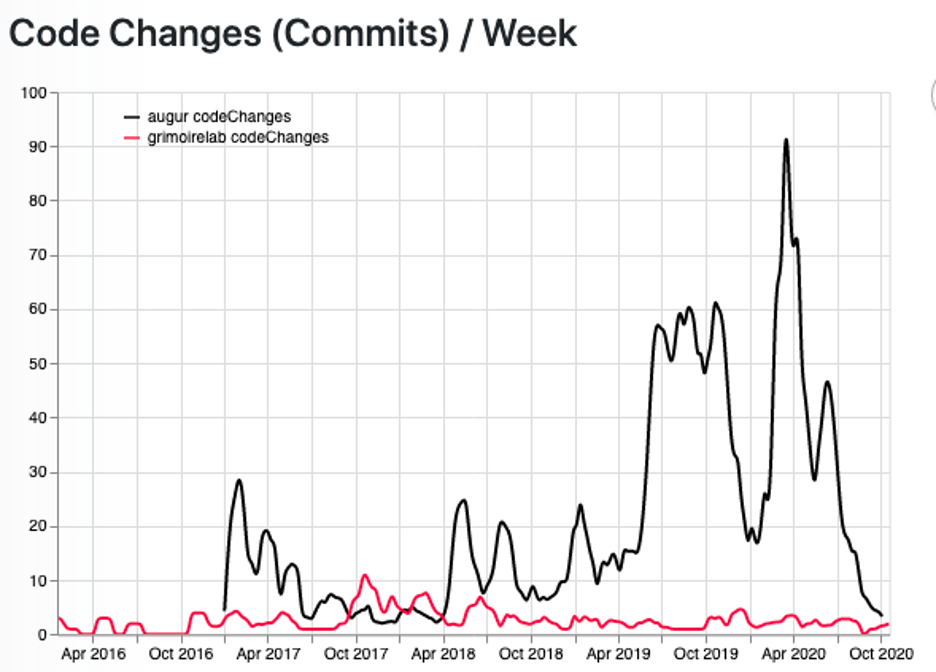
\includegraphics{images/burstiness_augur.png}

GrimoireLab:

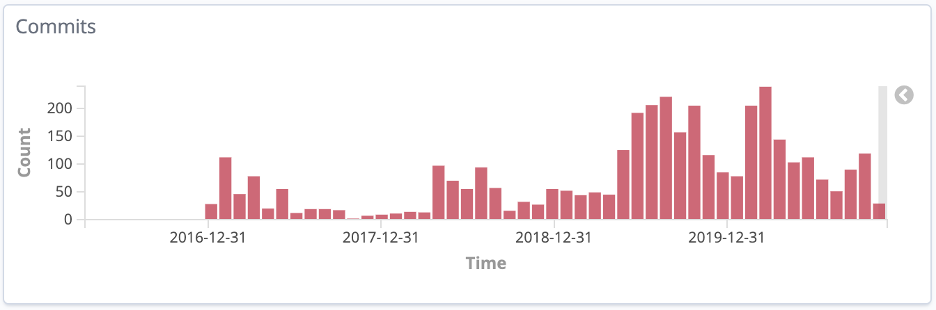
\includegraphics{images/burstiness_gl.png}

\hypertarget{ux63d0ux4f9bux5ea6ux91cfux7684ux5de5ux5177}{%
\subparagraph{提供度量的工具}\label{ux63d0ux4f9bux5ea6ux91cfux7684ux5de5ux5177}}

\begin{itemize}
\tightlist
\item
  Grimoire Lab
\item
  Augur
\end{itemize}

\hypertarget{ux6570ux636eux6536ux96c6ux7b56ux7565}{%
\subparagraph{数据收集策略}\label{ux6570ux636eux6536ux96c6ux7b56ux7565}}

\begin{itemize}
\item
  定量

  \begin{itemize}
  \tightlist
  \item
    基于时间框识别偏离某种常规状态的活动
  \item
    某些阈值的异常值,使用布林带等统计数据来衡量稳定性或波动性:
    \href{https://en.wikipedia.org/wiki/Bollinger_Bands}{https://en.wikipedia.org/wiki/Bollinger\_Bands}
  \end{itemize}
\item
  定性调查问题

  \begin{itemize}
  \tightlist
  \item
    为什么你在某一段时间内贡献量更多?
  \item
    你认为这些特有突发性波动的根本原因是什么?
  \item
    不同事件(例如, 黑客松,导师计划,或者会议)对项目活动有什么影响?
  \end{itemize}
\end{itemize}

\hypertarget{references}{%
\paragraph{References}\label{references}}

该指标的灵感来自 Goh 和 Barabasi (2008):
\href{https://arxiv.org/pdf/physics/0610233.pdf}{https://arxiv.org/pdf/physics/0610233.pdf}
